\newpage

\anonchapter{Лабораторная работа №1}
\setcounter{chapter}{1}
\setcounter{figure}{0}
\setcounter{table}{0}

\begin{center}
Измерение удельного электрического сопротивления полупроводников двухзондовым методом\\
(4 часа)
\end{center}

\section{Цель работы}
Определение распределения удельного сопротивления по длине прямоугольного образца монокристаллического кремния двухзондовым методом при комнатной температуре.

\section{Теоретическое введение}
\subsection{Удельное электросопротивление}
\paragraph{Характеристика удельного сопротивления полупроводников}

Фундаментальным законом, устанавливающим связь приложенного к проводящему образцу напряжения $U$ и протекающим в образце током $I$ является экспериментальный закон Ома:
\begin{equation}
I = \frac{U}{R}
\end{equation}
где $R$ - электросопротивление образца, является константой.

Электросопротивление $R$ зависит от геометрической формы и размеров образца, а также характеристики материала - удельного электросопротивления $\rho$. Для однородного образца правильной геометрической формы длиной $L$ и площадью поперечного сечения $S$
\begin{equation}
R = \rho \frac{L}{S}
\end{equation}

Если в этом случае выразить интегральные характеристики $U$ и $I$ через дифференциальные $j$ (плотность тока) и $\mathcal{E}$ (напряженность электрического поля), получаем закон Ома в дифференциальной форме
\begin{equation}
j = \frac{I}{S}, \mathcal{E} = \frac{U}{L} \rightarrow j = \frac{\mathcal{E}}{\rho} = \sigma \mathcal{E}
\end{equation}
где $\sigma$ - удельная электропроводность вещества.

В свою очередь, $\sigma$ определяется концентрацией свободных носителей заряда (СНЗ) $n$ и их подвижностью $\mu$:
\begin{equation}
\sigma = e n \mu
\label{UES}
\end{equation}

\begin{equation}
\mu = \frac{V_{\text{др}}}{\mathcal{E}}
\label{mu_from_Vdr}
\end{equation}
где $e = 1.6e^{-19}$ Кл - заряд электрона, $V_{\text{др}}$ - средняя дрейфовая скорость движения электрона под действием электрического поля.

Поведение $\sigma$ в кристаллических полупроводниках и металлах различно. Для металлов $\sigma$ - постоянная величина, в то время как в полупроводниках $\sigma$ зависит от примесного состава, кристаллического совершенства материала и внешних факторов — освещения, радиации и др. Эти материалы имеют также различный характер температурной зависимости удельной электропроводности.

Для полупроводников, у которых есть два типа СНЗ - электроны с концентрацией $n$ и дырки с концентрацией $p$ - формулу (\ref{UES}) необходимо дополнить:

\begin{equation}
\sigma = e n \mu_{n} + e p \mu_{p}
\end{equation}
где $\mu_{n}$ и $\mu_{p}$ - подвижость электронов и дырок соответственно.

\paragraph{Концентрация свободных носителей заряда}

Основой для понимания физических процессов и электрических явлений в твердом теле является зонная теория электронных спектров, базирующаяся на квантовомеханичеких представлениях. Концентрация свободных электронов — это концентрация занятых квантовомеханических состояний в зоне проводимости, а концентрация дырок — концентрация незаполненных состояний в валентной зоне. При температуре 0\textdegree К в полупроводнике свободных носителей заряда нет, в то время как концентрация электронов в металле практически не зависит от температуры и составляет величину порядка концентрации атомов металла в единице объема ($\approx 10^{22} \text{см}^{-3}$). СНЗ в полупроводниковых материалах появляются за счет термической генерации свободных носителей заряда (за счет энергии кристаллической решетки). Возможны несколько случаев:
\begin{enumerate}
\item переход электронов из валентной зоны в зону проводимости (в этом случае создаются одинаковые концентрации электронов и дырок $n = p = n_{i}$);
\item переход электронов из валентной зоны на уровень акцепторной примеси $E_{A}$, при этом создаются свободные дырки;
\item переход электронов с уровня донорной примеси $E_{\text{Д}}$ в зону проводимости (создаются свободные электроны).
\end{enumerate}

Верхний предел концентрации СНЗ при комнатной температуре в полупроводниках определяется пределом растворимости легирующих примесей ($\approx 10^{19} \text{см}^{-3}$), нижний предел определяется собственной концентрацией СНЗ - $n_{i}$.

Важнейшим параметром проводящего материала, однозначно связанным с концентрацией ННЗ, является уровень Ферми $F$. Для невырожденного материала
\begin{equation}
n = N_{c} \exp \left( -\frac{E_{c}-F}{k T} \right),
p = N_{v} \exp \left( -\frac{F - E_{v}}{k T} \right)
\end{equation}
где: $k$ – константа Больцмана, $N_{c}$ ($N_{v}$) — плотность состояний на дне зоны проводимости (потолке валентной зоны), зависящая от температуры и эффективной массы соответствующих СНЗ:
\begin{equation}
\begin{split}
%\begin{array}
N_{c} &= 2 \left( \frac{2 \pi m^{*}_{n} k T}{h^2} \right) = 4.82 \cdot 10^{15} \left( \frac{m^{*}_{n}}{m} \right)^{\frac{3}{2}} T^{\frac{3}{2}} = 2.5 \cdot 10^{19} \left( \frac{m^{*}_{n}}{m} \right)^{\frac{3}{2}} \left( \frac{T}{300} \right)^{\frac{3}{2}} \\
N_{v} &= 2 \left( \frac{2 \pi m^{*}_{pd} k T}{h^2} \right) = 2.5 \cdot 10^{19} \left( \frac{m^{*}_{pd}}{m} \right)^{\frac{3}{2}} \left( \frac{T}{300} \right)^{\frac{3}{2}}
%\end{array}
\end{split}
\end{equation}

Термодинамически равновесные концентрации $n$ и $p$ в невырожденном материале связаны соотношением:
\begin{equation}
n \cdot p = n_{i}^2 = N_{c} N_{v} \exp \left( -\frac{E_{g}}{2 k T} \right)
\end{equation}

При низких температурах доминирует процесс ионизации примеси, в области средних температур, к которой для большинства практически значимых полупроводниковых материалов относится комнатная температура, концентрация СНЗ равна концентрации легирующей примеси, и полупроводник является либо электронным либо дырочным. При дальнейшем повышении температуры примесный полупроводник становится собственным. Температура перехода к собственной проводимости тем выше, чем больше ширина запрещенной зоны и чем выше концентрация легирующих примесей в полупроводнике.

Легирующими или мелкими примесями в полупроводнике, являются примеси, энергия ионизации которых ($E_{c}$ — $E_{\text{Д}}$ для донорной примеси и $E_{\text{А}}$ — $E_{\text{v}}$ для акцепторной) сравнима со средней энергией кристаллической решетки в расчете на один атом — $kT$ ($0.025$ эВ). Для широкого круга алмазоподобных полупроводников такими примесями являются элементы, валентность которых отличается от валентности атомов полупроводникового материала на единицу. Так, для кремния и германия легирующими будут элементы III (акцепторы) и V (доноры) групп периодической системы Менделеева. Для соединений $A_{III}B_{V}$ – элементы II и VI групп. Элементы IV группы могут быть как донорами, так и акцепторами, в зависимости от того, элемент какой из подрешеток они замещают.

\paragraph{Подвижность свободных носителей заряда}

Для объяснения того факта, что электрическое поле вызывает в проводящей среде движение с постоянной скоростью (\ref{mu_from_Vdr}), а не ускорением, как это должно быть при действии силы величиной $e \mathcal{E}$ на частицу с массой $m$, в классической теории электропроводности было введено понятие среднего времени свободного пробега $\tau$ как величины, обратной вероятности столкновения электрона с решеткой. При таком столкновении энергия, полученная от электрического поля, отдается решетки и восстанавливается первоначальный импульс. В этом случае подвижность определяется выражением:
\begin{equation}
\mu = \frac{\mathcal{E} \tau}{m}
\label{mu_from_E}
\end{equation}

В рамках классической физики было непонятно, почему длина свободного пробега $L$ (произведение времени свободного пробега на тепловую скорость носителя заряда) составляет сотни параметров кристаллической решетки, т. е. почему при движении по кристаллической решетке электрон сталкивается только с одним из сотен атомов на его пути. Объяснить этот экспериментальный факт (как и ряд других, связанных в частности, с различием поведения электропроводности металлов и полупроводников) удалось в рамках квантовомеханической теории, точнее, зонной теории кристаллических твердых тел. Электрон как квантовомеханическая ферми-частица обладает не только энергий и импульсом, но и волновыми свойствами. Волновая функция электрона в периодическом поле идеальной кристаллической решетки периодически модулирована с периодом, равным постоянной решётки, что позволяет электрону двигаться без рассеяния. В идеальном кристалле время свободного пробега и подвижность были бы бесконечными. Однако идеальных кристаллических решеток не существует в принципе. При взаимодействии с локальными нарушениями периодического Кулоновского поля, создаваемого ядрами атомов, т. е. с дефектами кристаллической решетки, импульс электрона изменяется. К основным дефектам кристаллической решетки можно отнести тепловые колебания атомов, примесные атомы (нейтральные и ионизированные), дислокации, двойники и т.д.

При приложении электрического поля изменяется заполнение разрешенных квантовомеханических состояний. При выключении за счет взаимодействия с дефектами решетки система релаксирует, переходя в термодинамически равновесное состояние. Поэтому вводится понятие времени релаксации, которое в слабых электрических полях совпадает с введенным в классической теории электропроводности понятием времени свободного пробега и связано с подвижностью СНЗ выражением (\ref{mu_from_E}).

Подвижность СНЗ зависит от среднего времени релаксации возбужденного состояния, которое, в свою очередь, определяется механизмом рассеяния СНЗ. Термин «механизм рассеяния» отражает тот факт, что в результате столкновения с дефектами кристаллической решетки поток электронов (дырок) вдоль направления вектора напряженности электрического поля постепенно уменьшается (рассеивается), что приводит к исчезновению электрического тока после выключения электрического поля. Но процессы рассеяния идут и при протекании электрического тока. Чем больше концентрация дефектов кристаллической решетки, тем быстрее происходит процесс выбывания отдельных электронов из потока, определяющего электрический ток в материале, тем меньше среднее время релаксации, подвижность СНЗ и величина электропроводности. Каждому типу дефекта кристаллической решетки соответствует свой механизм рассеяния.

Квантовомеханические расчеты показывают, что даже при 0\textdegree К атомы совершают колебания (нулевые колебания). С ростом температуры амплитуда колебаний растет, и растет вероятность столкновения электронов с колеблющимися атомами. Квазичастицы с характерным набором частот и волновых функций, с которыми эти колебания происходят, называются фононами, поэтому во всех кристаллах будет иметь место механизм рассеяния на фононах (тепловых колебаниях атомов кристаллической решетки). Любой дефект кристаллической решетки (нейтральные и ионизированные примесные атомы, дислокации, малоугловые границы и границы зерен и т.д.) вызывает появление соответствующего механизма рассеяния. В полупроводниках, помимо рассеяния на фононах, характерного для металлов, может доминировать рассеяние на ионизированных атомах примеси, а при низких температурах — на нейтральных примесных атомах. В целом в данном кристалле имеется столько различных механизмов рассеяния, сколько типов дефектов кристаллической решетки. С каждым из них связана свой величина подвижности $\mu_{i}$. Подвижность для (\ref{UES}, \ref{mu_from_Vdr}) определяется по формуле:
\begin{equation}
\frac{1}{\mu} = \sum\limits_{i = 1}^{N}{\frac{1}{\mu_{i}}}
\end{equation}
где $N$ - число дефектов.

Наибольший вклад в величину подвижности вносит тот механизм, значение подвижности для которого минимально. Он определяется доминирующим типом дефектов.

Отличие поведения полупроводников и металлов связано с тем, что в металлах электронный газ является вырожденным, а в полупроводниках - невырожденным. Последние описываются классической статистикой Больцмана. Относительно слабый линейный рост удельного электросопротивления металлов с температурой связан с уменьшением подвижности при рассеянии на длинноволновых акустических фононах, в то время как активационный рост этого параметра у полупроводников определяется температурной зависимостью концентрации СНЗ. Освещение не влияет на электропроводность металлов. В полупроводниках при освещении светом с энергией квантов, превышающей ширину запрещенной зоны, происходит переход электрона из валентной зоны в зону проводимости, что увеличивает электропроводность. Это явление называется фотопроводимостью. Поэтому при определении электропроводности полупроводников образец необходимо затенять. Это требование особенно важно для высокоомных материалов, в которых концентрация СНЗ мала.

При анализе электрофизических свойств в проводящих материалах чаще используется понятие удельго электросопротивления. В частности, марка наиболее распространенного полупроводникового материала — кремния — включает значение $\rho$ при температуре 23\textdegree С, выраженное в $\text{Ом}\cdot\text{см}$. Так, марка КЭФ-20 означает кремний электронный, легированный фосфором, с удельным электросопротивлением $20$ $\text{Ом}\cdot\text{см}$ при комнатной температуре, КДБ 4.5 — кремний дырочный, легированный бором, с удельным электросопротивлением $4.5$ $\text{Ом}\cdot\text{см}$ при комнатной температуре.

\subsection{Методика измерения удельного электросопротивления полупроводников}

Для измерения удельного сопротивления полупроводниковых образцов используются контактные и бесконтактные методы.
Зондовые методы осуществляют прямое измерение сопротивления определенной области образца по величине падения напряжения на ней при протекании определенного электрического тока (переменного или постоянного). Эти измерения основаны на законе Ома и производятся по двухзондовой, однозондовой (сопротивление растекания), четырехзондовой методикам.
Бесконтактные высокочастотные методы основаны на зависимости свойств скин-слоя характеризующего глубину проникновения высокочастотного (ВЧ) или сверхвысокочастотного (СВЧ) электрического поля в образец от величины его электропроводности. По способу подключения образца к ВЧ измерительному контуру различают емкостные методики (образец становится частью измерительного конденсатора) или индуктивные методики (образец помещается в катушку индуктивности). В СВЧ методе измеряется относительное изменение СВЧ мощности в СВЧ волноводе при взаимодействии образца с СВЧ волной. В отличие от зондовых методов эти методики неразрушающие, однако в виду сложности расчетов они являются не абсолютными, а эталонными, то есть определение электропроводности образца производится при сравнении с его эталонным образцом. Бесконтактные высокочастотные методы в отличие от зондовых методов могут измерять удельное сопротивление и поликристаллических образцов, так как влияние существенно более высокоомных межкристаллитных прослоек слабо сказывается в высокочастотных измерениях.

\section{Методика двухзондовых измерений удельного электросопротивления}

\subsection{Сущность двухзондового метода}

Двухзондовый метод измерения удельного электросопротивления требует применения монокристаллических образцов правильной геометрической формы (удлиненный прямоугольный параллелепипед или цилиндрический стержень) с нанесенными на торцевые поверхности образца омическими контактами. Из всех методов измерения он является наиболее точным, но и наиболее трудоемким. В производстве он применяется на заводах по выращиванию поликристаллического кремния на специально выращенных для определения параметров материала слитках. Схема двухзондового метода измерений представлена на рисунке \ref{1_base_scheme}.

\begin{figure}[h!]\centering
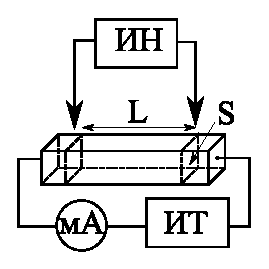
\includegraphics[height=4cm]{pic1_1.eps}
\caption{Принципиальная схема двухзондового метода измерения удельного сопротивления: ИТ – источник тока; ИН – измеритель напряжения; $L$ – расстояние между зондами; $S$ – площадь сечения образца}
\label{1_base_scheme}
\end{figure}

Если по образцу протекает электрический ток силой $I$, создающий благодаря постоянству сечения образца одинаковую плотность тока в любой точке образца, то, измерив падение напряжения U между эквипотенциальными поверхностями, на которые установлены зонды, можно найти удельное сопротивление $\rho$ по формуле
\begin{equation}
\rho = \frac{U S}{I L}
\end{equation}

При этом предполагается, что эквипотенциальные поверхности перпендикулярны вектору плотности тока и сопротивлением контактов «зонд-полупроводник» можно пренебречь. Если первое условие при небольших сечениях образца удовлетворить легко, то второе условие, как правило, не удовлетворяется в силу особенностей контактных явлений между металлом и полупроводником.

Сопротивление образца на участке $x$ равно
\begin{equation}
R(x) = \int\limits_{0}^{x} {\frac{\rho(x)}{S} d x}
\end{equation}

Для однородного образца $\rho = const$ и $R(x) = \frac{d x}{S}$ - линейная функция от расстояния $x$. Если образец неоднороден, то зависимость $R(x)$ нелинейна, а сопротивление $\rho(x)$ можно найти по формулам

\begin{equation}
\begin{split}
\rho(x) &= S \cdot \tg(\phi) \\
\tg(\phi) &= \frac{d R}{d x} = \frac{\Delta R}{\Delta L}
\end{split}
\label{1_rho}
\end{equation}

\subsection{Анализ паразитных явлений и методика их устранения в двухзондовых измерениях удельного электросопротивления}

Пренебрежение влиянием контактных явлений может привести к наиболее грубым ошибкам измерения удельного сопротивления двухзондовым методом. Поэтому остановимся на описании вклада этих явлений подробнее.

\paragraph{Переходное сопротивление контакта «зонд-полупроводник».}
Из-за потенциального барьера (контактной разности потенциалов) вольтамперная характеристика (ВАХ) контакта металл-полупроводник является нелинейной то есть сопротивление контакта зависит от величины и направления проходящего через него электрического тока. При измерении с помощью вольтметра падения напряжения между зондами в случае запирающих контактов, когда потенциальный барьер препятствует прохождению основных носителей заряда, один из контактов будет обладать высоким сопротивлением, которое может оказаться сопоставимым с внутренним сопротивлением вольтметра. Это внесет грубую ошибку в результат измерений. Избавиться от этой ошибки помогает компенсационный метод измерения падения напряжения, принципиальная схема которого представлена на рисунке \ref{1_potenc}. Для измерения падения напряжения используется потенциометр, представляющий собой калиброванный источник напряжения.

\begin{figure}[h!]\centering
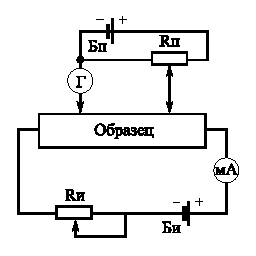
\includegraphics[height=4cm]{pic1_2.eps}
\caption{Схема потенциометрического метода измерения}
\label{1_potenc}
\end{figure}

С помощью потенциометра $R_{\text{п}}$ между измерительными зондами создается компенсирующее напряжение $\text{Б}_{\text{п}}$, равное по величине и противоположное по знаку измеряемому. Последовательно с потенциометром в измерительную цепь включается чувствительный нуль-гальванометр Г. Если компенсирующее и измеряемое напряжение $\text{Б}_{\text{и}}$ равны по величине, то нуль-гальванометр фиксирует равенство нулю электрического тока, протекающего через измерительные зонды. В этом случае даже при высоком переходном сопротивлении контакта «зонд-полупроводник» падение напряжения на этом переходном сопротивлении равно нулю ($U_{\text{зонд}} = I R_{\text{зонд}} = 0$, т.к. $I = 0$).

Здесь следует добавить два важных замечания. Во-первых, внутреннее сопротивление потенциометра шунтирует сопротивление образца в цепи электрического тока, текущего через образец от источника тока, поэтом всегда должно соблюдаться требование $R_{\text{п}} \gg R_{\text{образца}}$. С учетом этого применяются для различных диапазонов измеряемых сопротивлений высокоомные потенциометры постоянного тока (ППТВ). Во-вторых, если нуль-гальванометр показывает равенство тока нулю, то это может означать, что протекающий ток меньше предела чувствительности гальванометра. Поэтому если использовать для измерения падения напряжения прибор, потребляющий электрический ток не выше предела чувствительности гальванометра, то он может заменить компенсационную схему измерения (то есть? обеспечить ту же погрешность измерения за счет вклада переходного сопротивления контактов).

\paragraph{Вклад паразитных термоЭДС.}

При измерении на высоких токах вдоль образца может возникать паразитная термоЭДС. Причиной появления термоЭДС является градиент температуры, возникающий при неравномерном разогреве образца за счёт протекающего тока. Знак этого градиента температуры не зависит от направления электрического тока. Благодаря этому такая термоЭДС может легко быть исключена из данных измерений при проведении двух измерений падения напряжения $U_{1}^{+}$ и $U_{2}^{-}$ между зондами при двух различных направлениях электрического тока. Падение напряжения на образце $U_{\text{обр}}$ и величину термоЭДС можно найти, определяя полусумму или полуразность величин $U_{1}^{+}$ и $U_{2}^{-}$ с учётом их знака.

\begin{equation}
\begin{split}
U_{1}^{+} &= I R_{\text{обр}} + U_{\text{ТЭДС}} \\
U_{2}^{-} &= -I R_{\text{обр}} + U_{\text{ТЭДС}} \\
U_{\text{обр}} &= I R_{\text{обр}} = \frac{U_{1}^{+} - U_{2}^{-}}{2} \\
U_{\text{ТЭДС}} &= \frac{U_{1}^{+} + U_{2}^{-}}{2}
\end{split}
\label{Uteds}
\end{equation}

Если токовые контакты не являются омическими, то при прохождении тока в них может возникать эффект Пельтье, то есть нагревание или охлаждение контакта в зависимости от направления тока. ТермоЭДС, создавшуюся в результате такого градиента температуры, вышеописанным способом устранить невозможно, так как она будет изменять знак с изменением направления тока. Неомичность токовых контактов также может привести к возникновению взаимосвязанных явлений инжекции, эксклюзии, экстракции и аккумуляции в приконтактных областях образца, которые могут изменить истинную величину электросопротивления. Следует делать минимальной величину тока, протекающего в образце, чтобы избежать разогрева образца, а также защищать образец от освещения во избежание возникновения в нем фотопроводимости или контактных фотоэдс. Все эти явления могут давать существенную погрешность измерения в высокоомных образцах.

\section{Описание измерительной установки}

Принципиальная электрическая схема установки показана на рисунке \ref{1_scheme}

\begin{figure}[h!]\centering
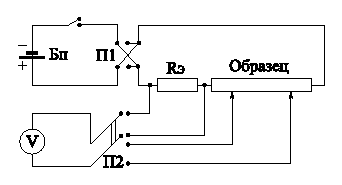
\includegraphics[height=4cm]{pic1_3.eps}
\caption{Принципиальная схема измерений двухзондовым методом}
\label{1_scheme}
\end{figure}

Величина электрического тока через образец устанавливается при помощи управляемого линейного источника питания Б5-30. Точное определение тока производится по измерению падения напряжения $V$ на эталонном сопротивлении $R_{\text{э}}$, включённом последовательно с сопротивлением образца $R_{\text{обр}}$. Переключатель П2 может подключать вольтметр В7-21А или к образцу, или к эталонному сопротивлению. Переключатель П1 меняет направление электрического тока в образце. Источник тока может быть заменён батареей с подключённым последовательно переменным сопротивлением.

Исследуемый образец с нанесенным омическими контактами помещается в токовые зажимы на предметном столе в поле зрения оптического микроскопа. Определение расстояния между измерительными зондами производится с помощью микрометрической головки микроскопа. Нулевое положение устанавливается при совмещении перекрестия в поле зрения микроскопа с изображениями соприкасающихся первого и второго зондовых контактов. Полный оборот микрометрической головки микроскопа соответствует перемещению перекрестия на 1 мм.

Для определения типа проводимости образца применяется метод термозонда, принципиальная схема которого изображена на рисунке \ref{1_condtype}. Образец помещается на массивную металлическую пластину, служащую «холодным» контактом. Вместо массивного основания можно использовать холодный щуп. Нагретым с помощью небольшого электронагревателя зондом касаются верхней поверхности образца. Если образце имеет место проводимость n-типа, то электроны в образце диффундируют от нагреваемой термозондом верхней грани к «холодной» нижней грани, заряжая ее отрицательно. Верхняя грань образца будет заряжаться положительно за счет остающихся нескомпенсированными ионов донорной примеси $N_{D}^{+}$. Если образец имеет p-тип проводимости, то к «холодной» грани образца диффундируют положительно заряженные дырки, оставляя на «горячей» грани отрицательный заряд $N_{A}^{-}$ нескомпенсированных ионов акцепторов. Если в качестве регистрирующего устройства между горячим и холодным зондом включить параллельно светодиоды разного цвета, то при изменении типа проводимости измениться направление тока в цепи диодов и включится тот, напряжение на котором будет прямым. В используемом в работе детекторе в образце n-типа проводимости загорается зеленый светодиод, в образце p-типа — красный.

\begin{figure}[h!]\centering
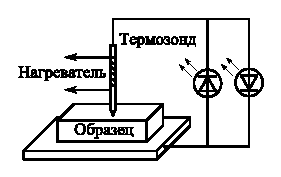
\includegraphics[height=4cm]{pic1_4.eps}
\caption{Принципиальная схема измерений двухзондовым методом}
\label{1_condtype}
\end{figure}

\section{Порядок проведения работы и указания по технике безопасности}

\begin{enumerate}
\item Измерить толщину и ширину образца.
\item Установить образец на предметном столике и опустить на его поверхность измерительные зонды достаточно далеко от токовых контактов.
\item Установить необходимую величину тока через образец.
\item Привести в соприкосновение оба зонда, отметить нулевую точку отсчета на микрометрической головке микроскопа.
\item Повернуть микрометрическую головку микроскопа на 360\textdegree, переместить подвижный зонд на 1 мм по поверхности образца (конец зонда должен совместиться с перекрестьем в поле зрения микроскопа).
\item Измерить величину $U_{1}^{+}$ и $U_{2}^{–}$ с освещением и без освещения образца. Занести данные в таблицу \ref{1_table}.
\item Повторить п.п. 5 и 6.
\item Рассчитать зависимость $U_{\text{обр}}$ от расстояния $L$.
\item Изменить величину тока через образец и повторить измерение $U_{\text{обр}}$ от расстояния $L$.
\end{enumerate}

Электрический ток в измерительной схеме не превышает 3мА.

\section{Обработка результатов эксперимента}

\begin{enumerate}
\item Результаты измерений занести в таблицу, отметив условие освещённости образца.
\item Построить графики $R_{\text{обр}} = f(L)$ и $U_{\text{ТЭДС}} = f(L)$.
\item В соответствии с формулами (\ref{1_rho}) рассчитать $\rho(x)$.
\item Построить график $\rho(L)$ и сопоставить его с графиком $U_{\text{ТЭДС}}(L)$. Выполнить это построение для различных значений тока через образец и условий его освещенности.
\item Рассчитать погрешность измерения сопротивления Rобр и l и нанести их на графики.
\item Оценить погрешность определения удельного сопротивления $\delta \rho$.
\item Высказать суждение об однородности или неоднородности образца и влиянии величины электрического тока через образец и условий его освещенности на результаты измерений.
\end{enumerate}

\begin{table}[h!]
\caption{Измерение удельного электросопротивления при освещении (без освещения)}
\begin{center}
\begin{tabular}{c|c|c|c|c|c|c|c|c}
№ & $L$ & $U_{\text{э}}$ & $I = \frac{U_{\text{э}}}{R_{\text{э}}}$ & $U_{1}^{+}$ & $U_{2}^{-}$ & $U_{\text{обр}}$ & $U_{\text{ТЭДС}}$ & $R_{\text{обр}}$ \\
\hline
& мм & мВ & мА & мВ & мВ & мВ & мВ & Ом \\
\hline
\end{tabular}
\end{center}
\label{1_table}
\end{table}

\section{Контрольные вопросы}
\begin{enumerate}
\item Почему для определения удельной электропроводности полупроводниковых материалов применяют зондовые методы?
\item Достоинства и недостатки двухзондового метода измерения удельной электропроводности полупроводниковых материалов.
\item Как определить удельное сопротивление однородного и неоднородного образца при измерении двухзондовым методом?
\item Механизмы электропроводности в полупроводниках и металлах.
\item Какими факторами определяется величина концентрации свободных носителей заряда в полупроводниках и металлах при комнатной температуре?
\item Чем определяется температурная зависимость электропроводности полупроводников и металлов?
\item Какие процессы определяют появление свободных носителей заряда в области собственной и примесной проводимости?
\item От каких факторов зависит температура перехода от примесной проводимости к собственной?
\item Какие примеси создают n- или p- проводимость в полупроводнике?
\item Как влияет освещение на электропроводность полупроводников?
\item Какие материалы при измерении электропроводности необходимо затенять и почему?
\item Понятие механизма рассеяния свободных носителей заряда.
\item Назовите основные механизмы рассеяния свободных носителей заряда в полупроводниках и металлах.
\item В чем проявляется отличие свойств свободного электронного газа полупроводников и металлов?
\item Как влияет кристаллическое совершенство материала на электропроводность полупроводников и металлов?
\end{enumerate}

\section{Литература}
\begin{enumerate}
\item К.В. Шалимова. Физика полупроводников. СПб.: Лань, 2011 г.
\item В.В. Батавин, Ю.А. Концевой, Ю.В. Федорович. Измерение параметров полупроводниковых материалов и структур. М.: Радио и связь, 1985 г.
\item Л.П. Павлов. Методы определения основных параметров полупроводниковых материалов. М.: Высшая школа, 1975 г.
\item В.В. Горбачев, Л.Г. Спицина. Физика полупроводников и металлов. М.: Высшая школа, гл. 1, 1986 г.
\end{enumerate}